\documentclass[a4paper,11pt]{report}
%
%--------------------   start of the 'preamble'
%
\usepackage{graphicx,amssymb,amstext,amsmath,hyperref,color}
%
%%    homebrew commands -- to save typing
\newcommand\etc{\textsl{etc}}
\newcommand\eg{\textsl{eg.}\ }
\newcommand\etal{\textsl{et al.}}
\newcommand\Quote[1]{\lq\textsl{#1}\rq}
\newcommand\fr[2]{{\textstyle\frac{#1}{#2}}}
\newcommand\miktex{\textsl{MikTeX}}
\newcommand\comp{\textsl{The Companion}}
\newcommand\nss{\textsl{Not so Short}}
\begin{document}
%%%%%%%%%%%%%%%%%%%%%%%%%%%%%%%%%%%%%%%%%%%%%%%%%%%%%%%%%%
%%%%%%%%%%%%    Color Definition      %%%%%%%%%%%%%%%%%%%

%\usepackage{color}
%\definecolor{black}{named}{Black}  
%\definecolor{blue}{named}{Periwinkle}  %BLUE
%\definecolor{orange}{named}{YellowOrange} %orange
%\definecolor{orange}{named}{Black}
%\definecolor{cyan}{named}{Black}

%%%%%%%%%%%%%%%%%%%%%%%%%%%%%%%%%%%%%%%%%%%%%%%%%%%%%%%%%%%
%%%%%%%%%%%%%%%%%%%%%%%%%%%%%%%%%%%%%%%%%%%%%%%%%%%%%%%%%%%

\thispagestyle{empty}
\begin{center}

\begin{table}[h]
\centering
\begin{tabular}{lr}
\LARGE The LNM Institute of Information Technology & 
\includegraphics [width=0.20\textwidth]{lnmiit.jpg}
\end{tabular}
\end{table}
\vspace{1cm}
%{\LARGE Data Centres}
\vspace{1cm}
{\LARGE \bf Performance Analysis and Optimization }\vspace{.05in}\\
{\LARGE \bf of Individualised CPU-GPU Core }\vspace{.05in}\\
{\LARGE \bf Systems }\vspace{.05in}\\

\vspace{1cm}
{A report submitted for the Operating Systems}\\
\vspace{3cm}
%\done by
\normalsize Done by \\
\vspace{1cm}
\begin{table}[h]
\centering
\begin{tabular}{lr}\hline \\
Names of Students & Roll No\\ \\ \hline
\\
Anshul Gupta & Y11UC047 \\
Ashish Agarwal & Y11UC062\\ 
Nikunj Gupta & Y11UC155\\
P Sai Krishna & Y11UC159 \\
Parvinder Singh Kalsi & Y11UC161\\ \\ \hline 
\end{tabular}
\end{table}
\vspace{2cm}
{Submitted on : April 16,2013}\\
\vspace{1cm}
\end{center}

\newpage
{\bf \LARGE Preface}
\vspace{3cm}
\label{preface}

This project \textbf{"Performance Analysis and Optimization of Individualised CPU-GPU Core Systems"} has been undertaken keeping in minds the heights "Information Technology has reached" and when everything is powered with computers does make a great difference. \\

Initially, the CPUs are responsible for handling all of the computing and instructions that it receives from the user and the system. However, with the increaseof technology and the demand of technology, it was best to take some of the pressure of the CPU and give it other processors. In comparison to CPUs, GPUs have more transistors that can handle more work and offers greater resolutions. Most of the GPUs transistors perform calculation related to 3D technologies. They wereoriginally used to accelerate the memory-intensive work of texturemapping and rendering polygons. Many GPUs also support technologies for advanced gaming or digital playback, offering better and advanced systems. \\

%\end{center}

\newpage
{\bf \LARGE Acknowledgement}
\vspace{3cm}


We would like to take opportunity to express our humble gratitude to Prof. Gaurav Somani who motivated and guided us to executed this project. His constant guidance and willingness to share his vast knowledge made us understand this project and its manifestations in great depths and helped us to work on the tasks assigned to us. \\
 
We are highly thankful to our project internal guide Miss. Anamika Sharma whose invaluable guidance helped us understand the project better. \\

Although there may be many who remain unacknowledged in this humble note of gratitude there are none who remain unappreciated.

\vspace{3cm}
{\it April 2013}

\newpage
{\bf \LARGE Abstract}
\vspace{3cm}
\label{preface}

Today's supercomputers are computers of tomorrow and GPU processors are bridge between them today. \textbf{A graphics processing unit} or \textbf{GPU} is a specialized processor that offloads 3D or 2D graphics rendering from the microprocessor.\\\\

\textbf{ GPU computing} is the use of aGPU to do general purpose scientific andengineering computing. The model for GPU computing is to use a CPU and GPU together in a heterogeneous computingmodel. The sequential part of the application runs on the CPU and the computationally-intensive part runs on the GPU. From the user¶s perspective, the application just runs faster because it isusing the high-performance of the GPU to boost performance. Computing is evolving from"central processing" on the CPU to "co-processing" on the CPU and GPU. To enable this newcomputing paradigm, \textbf{NVIDIA invented the CUDA (Compute Unified Device Architecture)} parallel computing architecture.\\\\

The \textbf{NVIDIA \textregistered Tesla 20-series} is designed from the groundup for high performance computing. Based on the next generation CUDA GPU architecture. When compared to the latest quad-core CPU, Tesla 20-series GPU computingprocessors deliver equivalent performance at \textbf{1/20th the power consumption and 1/10th the cost} i.e. \textbf{it gives thepower of super computer in a pc based workstation.} 

\newpage
{\bf \LARGE Hardware Specifications}\\\\\\\\\\

\textbf{GPU : Nvidia Tesla C2050}\\
FORM FACTOR : 9.75” PcIe x16 form factor\\
Number Of Tesla GPUs: 1\\
Number of CUDA cores: 448\\
Frequency of CUDA cores: 1.15 GHz\\
Double Precision Floating Point Performance (Peak):  515 Gflops\\
Single Precision Floating Point Performance (Peak):  1.03 Tflops\\  
Total Dedicated: 3 GB GDDR5\\
Memory Speed: 1.5 GHz\\
Memory Interface:  384-bit\\
Memory Bandwidth:  144 GB/sec\\
Power Consumption:  238W TDP\\
System Interface:  PCIe x216 Gen2\\
Display Support:  Dual-Link DVI-I:1\\
Maximum Display Resolution: 60Hz, 2560x1600\\

\textbf{CPU : Intel® Xeon® Processor E5630}\\ 
Number  of Cores    : 4\\
Number of Threads   : 8\\
Clock Speed         : 2.53 GHz\\
Max Turbo Frequency : 	2.8 GHz\\
Intel® Smart Cache  : 	12 MB\\
Intel® QPI Speed    :	5.86 GT/s\\
Number of QPI Links : 	2\\
Instruction Set     : 	64-bit\\
Instruction Set Extensions: SSE4.2\\
Lithography: 32 nm\\
Max TDP : 80 W\\
VID Voltage Range: 0.750V-1.350VPU\\

\textbf{GPU : Nvidia GeForce GT 525M}
CUDA Cores: 96\\
Processor Clock Tester(MHz):  1200 MHz\\
Texture Fill Rate (billion/sec):  9.6\\
Memory Clock:  900 Mhz\\
Memory Interface:  DDR3\\
Memory Interface Width: 128-bit\\
Memory Bandwidth: 28.8\\

\textbf{CPU : Intel® Core™ i5-2450M Processor}\\
Number  of Cores: 2\\
Number of Threads: 4\\
Clock Speed: 2.5 GHz\\
Max Turbo Frequency: 3.1 GHz\\
Intel® Smart Cache: 3 MB\\
DMI: 5 GT/s\\
Instruction Set: 64-bit\\
Instruction Set Extensions: AVX\\
Lithography: 32 nm\\
Max TDP: 35 W\\

\textbf{GPU : Nvidia Geforce GT 630m}\\
CUDA Cores: 96\\ 
Graphics Clock (MHz): 800 MHz\\
Texture Fill Rate (billion/sec): Up to 12.8\\
Memory Interface: DDR3 \ GDDR5\\
Memory Interface Width: Up to 128bit\\
Memory Bandwidth (GB/sec): Up to 32.0\\
Bus Support: PCI Express 2.0\\
Maximum Digital Resolution: Up to 2560x1600\\

\textbf{CPU : Intel® Core™ i7-3610QM Processor}\\
Number of Cores: 4\\
Number  of Threads : 8\\
Clock Speed: 2.3 GHz\\
Max Turbo Frequency: 3.3 GHz\\
Intel® Smart Cache: 6 MB\\
DMI: 5 GT/s\\
Instruction Set: 64-bit\\
Instruction Set Extensions: AVX\\
Lithography: 22 nm\\
Max TDP: 45 W\\

\tableofcontents
%-----------------------------------------------------------
\chapter{Introduction}

\section{Introduction to GPU}
A \textbf{Graphics Processing Unit (GPU)}, also occasionally called \textbf{visual processing unit (VPU)}, is a specialized electronic circuit designed to rapidly manipulate and alter memory to accelerate the building of images in a frame buffer intended for output to a display. GPUs are used in embedded systems, mobile phones, personal computers, workstations, and game consoles. Modern GPUs are very efficient at manipulating computer graphics, and their highly parallel structure makes them more effective than general-purpose CPUs for algorithms where processing of large blocks of data is done in parallel. In a personal computer, a GPU can be present on a video card, or it can be on the motherboard or—in certain CPUs—on the CPU die. \\\\

\section{Introduction to CUDA}

\textbf{CUDA} also known as \textbf{Compute Unified Device Architecture} is a parallel computing platform and programming model created by NVIDIA and implemented by the graphics processing units (GPUs) that they produce. CUDA gives developers access to the virtual instruction set and memory of the parallel computational elements in CUDA GPUs. Using CUDA, the latest Nvidia GPUs become accessible for computation like CPUs. Unlike CPUs, however, GPUs have a parallel throughput architecture that emphasizes executing many concurrent threads slowly, rather than executing a single thread very quickly. This approach of solving general-purpose (i.e., not exclusively graphics) problems on GPUs is known as GPGPU.


\chapter{Initial Findings}

\section{How CPUs and GPUs differ ?}
\begin{enumerate}
\item Latency Intolerance versus Latency Tolerance
\item Task Parallelism versus Data Parallelism
\item Multi-threaded Cores versus SIMT (Single Instruction Multiple Thread) Cores
\item 10s of Threads versus 10,000s of Threads
\end{enumerate}

\section{Latency and Throughput}
\begin{enumerate}
\item “Latency is a time delaybetween the moment something is initiated, 
and the moment one of its effects begins or becomes detectable”
\item For example, the time delay between a request for texture reading and texture 
data returns
\item Throughput is the amount of work done in a given amount of time
\item For example, how many triangles processed per second
\item CPUs are low latency low throughput processors
\item GPUs are high latency high throughput processors
\end{enumerate}

\section{Latency}
GPUs are designed for tasks that can tolerate latency
\begin{enumerate}
\item Example: Graphics in a game (simplified scenario): 
\item To be efficient, GPUs must have high throughput, i.e. processing millions of pixels in a single frame
\end{enumerate}

\section{CPUs are designed to minimize latency}
\begin{enumerate}
\item Example: Mouse or keyboard input
\item Caches are needed to minimize latency
\item CPUs are designed to maximize running operations out of cache
\item Instruction pre-fetch
\item Out-of-order execution, flow control
\item ÆCPUs needa large cache, GPUs do not
\item GPUs can dedicate more of the transistor area to computation horsepower
\end{enumerate}

\section{Parallism in GPU v. GPU}
\subsection{CPU}
\begin{enumerate}
\item CPUs use task parallelism.
\item Multiple tasks map to multiple threads.
\item Tasks run different instructions.
\item 10s of relatively heavyweight threads run on 10s of cores.
\item Each thread managed and scheduled explicitly.
\item Each thread has to be individually programmed. 
\end{enumerate}
\subsection{GPU}
\begin{enumerate}
\item GPUs use data parallelism.
\item SIMD model (Single Instruction Multiple Data).
\item Same instruction on different data.
\item 10,000s of lightweight threads on 100s of cores.
\item Threads are managed and scheduled by hardware.
\item Programming done for batches of threads (e.g. one pixel shader per group of pixels, or draw call).
\end{enumerate}
\section{Why are we still using CPUs instead of GPUs?}
GPUs have far more processor cores than CPUs, but because each GPU core runs significantly slower than a CPU core and do not have the features needed for modern operating systems, they are not appropriate for performing most of the processing in everyday computing.Features missing from GPUs include interrupts and virtual memory, which are required to implement a modern operating system. Furthermore, GPUs use a fundamentally different architecture; one would have to program an application specifically for a GPU for it to work, and significantly different techniques are required to program GPUs. The GPU is not faster than the CPU. The CPU excels at doing complex manipulations to a small set of data, the GPU excels at doing simple manipulations to a large set of data.\\\\
The reason why we are still using CPU is not because x86 is the king of CPU architecture and Windows is written for x86, the reason why we are still using CPU is because the kind of tasks that an OS needs to do, i.e. making decisions, is run more efficiently on a CPU architecture. An OS needs to look at a number of different types of data and make various decisions which all depends on each other; this kind of job does not easily parallelizes, at least not into an SIMD architecture.

\chapter{Problems faced while Installation}

\section{How to install NVidia driver in Fedora 18}
-------------------------------------------------------------------------------------------------

Fedora 18 comes with open source \textbf{NOUVEAU driver} for NVIDIA graphics card. To install the NVIDIA propriteray driver follow the below steps.

\begin{enumerate}
\item Blacklist the nouveau driver: Add below line to /etc/modprobe.d/blacklist.conf file blacklist nouveau.
\item Rebuild the initramfs image file using dracut:\\
* Backup the initramfs file
\begin{verbatim}
$ sudo mv /boot/initramfs-(uname -r).img /boot/initramfs-(uname -r).img.bak
\end{verbatim}
* Rebuild the initramfs file
\begin{verbatim}
$ sudo dracut -v /boot/initramfs-(uname -r).img (uname -r)
\end{verbatim}
\item Reboot the system to runlevel 3 (without graphics)
\item Check that nouveau driver is not loaded
\begin{verbatim}
$ lsmod | grep nouveau
\end{verbatim}
\item Run the NVidia driver package
\begin{verbatim}
$ sudo ./NVIDIA-Linux-x86\_64-195.36.15-pkg2.run
\end{verbatim}
Above command will create xorg.conf file in /etc/X11 directory which is responsible to use NVidia driver in X.
\item Restart the system and NVidia driver will be used now.
\end{enumerate}

\section{How to install NVidia driver in Fedora 18}
-------------------------------------------------------------------------------------------------

\begin{enumerate}
\item Get the latest NVIDIA driver from here. Reboot with run-level 3 and install the driver. This should be pretty much straight-forward. Reboot after install.
\item Get the latest CUDA Toolkit.
\item Install the toolkit. This is a little bit tricky as the installer will claim that you have the wrong GCC version. In order to overcome this problem, run the installer with
\begin{verbatim}
>sh cuda_5.0.35_linux_64_fedora16-1.run -override compiler
\end{verbatim}
Skip the driver installation and select [y] for the toolkit and sample files.
\item Although in step (3) the GCC version check has been skipped, it is still hard-coded in one of the CUDA header files. Thus, go to line 80 of
\begin{verbatim}
/usr/local/cuda-5.0/include/host_config.h \end{verbatim} (or wherever the installer has put this header file) and change
\begin{verbatim}
#if __GNUC__ > 4 || (__GNUC__ == 4 && __GNUC_MINOR__ > 6)
    to
#if __GNUC__ > 4 || (__GNUC__ == 4 && __GNUC_MINOR__ > 7)
\end{verbatim}
Now NVCC won’t complain about this.
\item When you try to compile your project NVCC still claims about this
\begin{verbatim}
... atomicity.h(48): error: identifier "__atomic_fetch_add" is undefined
... atomicity.h(52): error: identifier "__atomic_fetch_add" is undefined
\end{verbatim}
We found a nice workaround for this problem here. All you need to do is
\begin{verbatim}
> echo "#undef _GLIBCXX_ATOMIC_BUILTINS" 
  > /usr/local/include/undef_atomics_int128.h
> echo "#undef _GLIBCXX_USE_INT128" 
  >> /usr/local/include/undef_atomics_int128.h
\end{verbatim}
and include this file when compiling with NVCC, i.e.
\begin{verbatim}
> nvcc.bin --pre-include /usr/local/include/undef_atomics_int128.h
  [other commands]
\end{verbatim}
Done. That worked for me, and I could compile the examples (after modifying the Makefiles with the “--pre-include” trick from (5)” without any troubles. Results from the NVIDIA samples look reasonable, what makes me think that CUDA 5.0 should work without (large) troubles on F18.\\
\begin{verbatim}
After following the steps above you may need to do the following
to build the examples.

A) The Makefiles don't pay attention to LD_LIBRARY_PATH or 
the ldconfig.
Assuming you installed to /usr/local, they use the path 
/usr/local/cuda/lib64 
but disregard the /usr/lib64/nvidia/ directory in which the libcuda*so
is located. To fix ad a symlink in the /usr/local/cuda/lib64 directory:
$ cd /usr/local/cuda/lib64
$ ln -s /usr/lib64/nvidia/libcuda.so libcuda.so

B) Run make from the /usr/local/cuda/samples directory as follows:
$ cd /usr/local/cuda/samples
$ make -k EXTRA_NVCCFLAGS=
"--pre-include /usr/local/include/undef_atomics_int128.h"
where /usr/local/include/undef_atomics_int128.h is the header file 
constructed in the previous post.
The "-k" tells make to continue even if a particular example fails to build,
e.g. for examples requiring something you don't have installed such as mpi. 
\end{verbatim}
\end{enumerate}

\chapter{Benchmark-I}

\section{The Task}
The objective of the program is simple. It generates an array up to a certain length of integers. It then computes the square roots of these, saving them to another array of the same length. This operation it performs on both the CPU and the GPU, and reports the process times taken on the two and their ratio. These three numbers are measured for a range of process size (total number of operations required for the process).
Therefore, with the array size fixed, the task is instead repeated, i.e. square roots of the same first array are computed and repeatedly saved to the second array, replacing the identical values before. In terms of utility this operation is an unproductive repetition, but in terms of analysing optimization, which is our goal, this serves equally well as any other, more utilitarian method of lengthening the process. In fact, increasing the array size would have meant computing square roots of increasingly larger numbers, which is not a proportional
increase in task size. However, repeating the same computation is a linear way to increase the task size, and thus the results may conveniently be plotted on a linear scale. The repetition loop is lengthened in steps of 100. For each length of the loop, process times on the GPU, CPU and their ratio are measured for 10 samples, and the average of each is written to a file.

\section{Code Walkthrough}
Code Walkthrough mentioned in file codewalkthrough.

\section{Results}

\subsection{Output}
The program displays information from each sample on screen, but writes only the statistics from each sampling to file, without information from all the samples. The first allows easy debugging, while the second allows easy analysis and plotting of the final data.\\\\
The Outputs have been mentioned in the following files :\\\\
\begin{enumerate}
\item samplevsgpu for GPU Result
\item samplevscpu for CPU Result
\item samplevsratio for GPU-CPU Ratio
\item time.txt for Time
\end{enumerate}

\subsection{Plots}
\vspace{1cm}
\textbf{CPU Process Times}\\\\
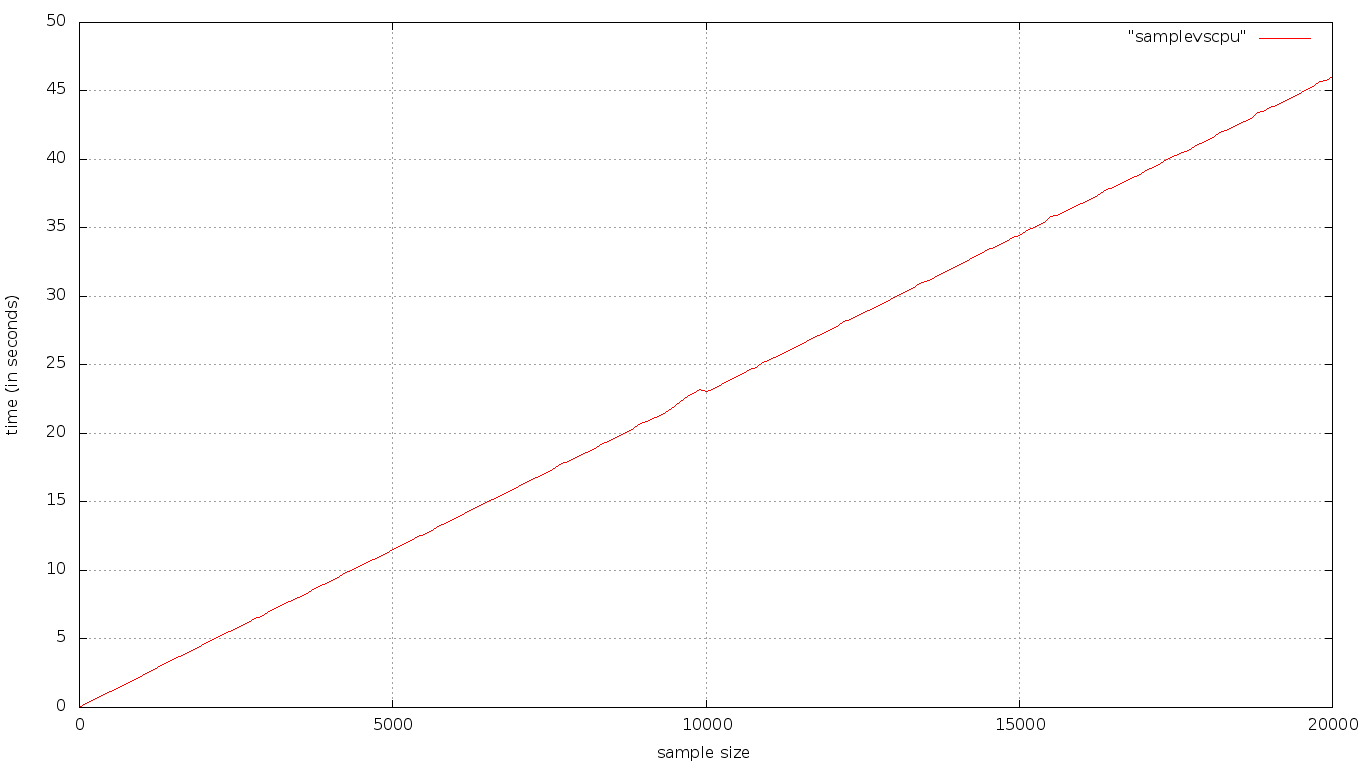
\includegraphics [width=1.2\textwidth]{cpu.png}
\newpage
\textbf{GPU Process Times}\\\\
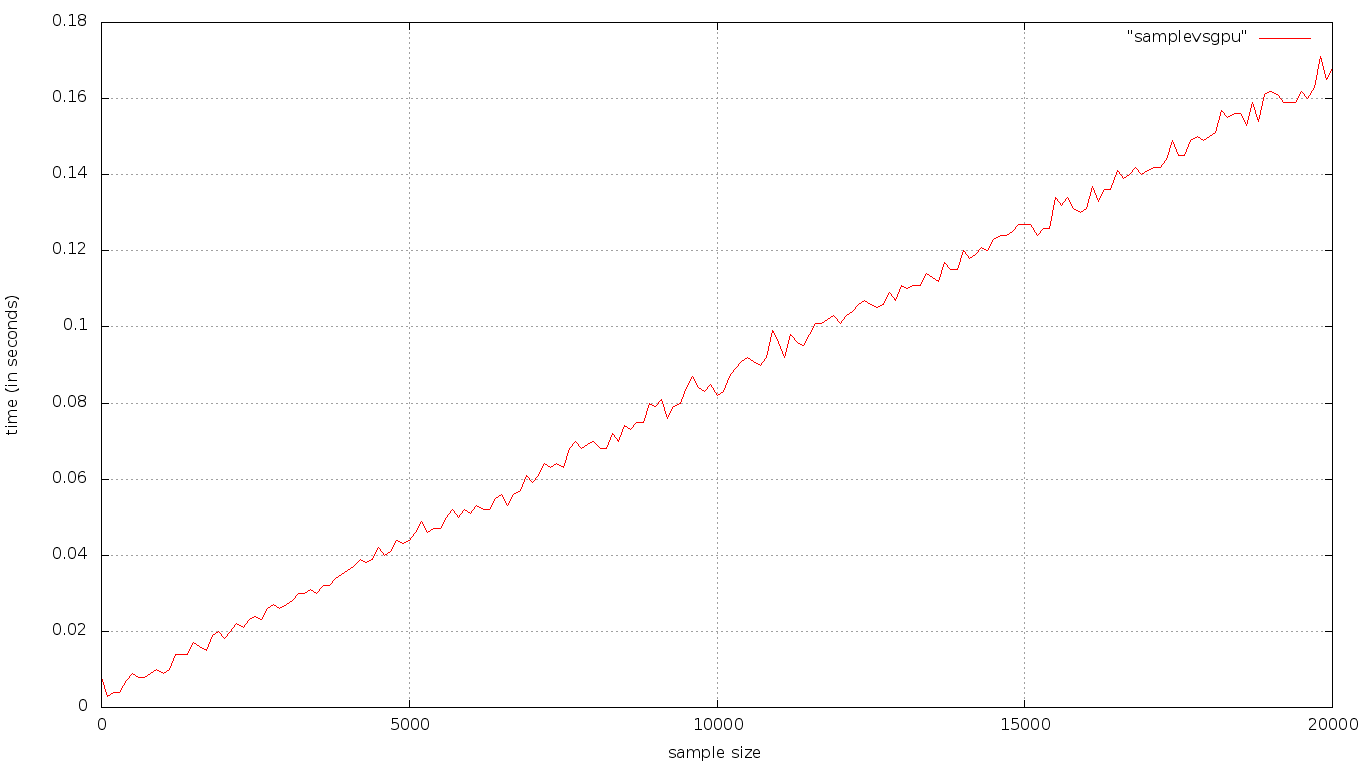
\includegraphics [width=1.2\textwidth]{gpu.png}
\textbf{CPU / GPU Ratio}\\\\
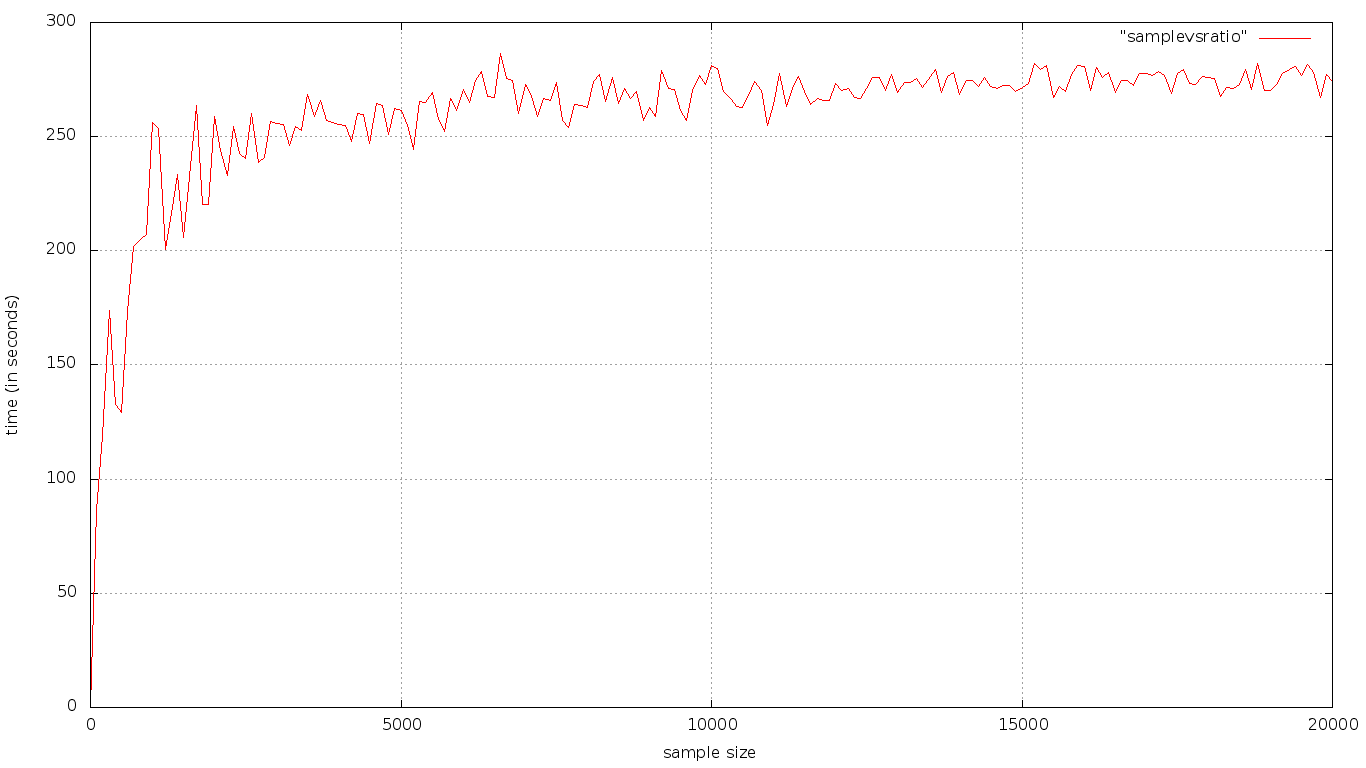
\includegraphics [width=1.2\textwidth]{ratio.png}

\section{Inferences}
\begin{enumerate}
\item For smaller tasks, the GPU is not much faster than the CPU as the data transfer overhead between host and device costs more than time saved by parallelization.
\item The ratio between GPU and CPU speeds, however, does not keep rising with increasing task size. It reaches an asymptote of about a 280-fold efficiency. This occurs when the transfer overheads take negligible time compared to that taken by the actual arithmetical computations on the device.
\item The above code follows \href{http://en.wikipedia.org/wiki/Amdahl's_law}{Amdahl's Law} The speedup of a program using multiple processors in parallel computing is limited by the sequential fraction of the program. For example, if 95\% of the program can be parallelized, the theoretical maximum speedup using parallel computing would be 20× as shown in the diagram, no matter how many processors are used.
\end{enumerate}

\chapter{Benchmark-II}

\section{The Task}
The objective of the program is simple. The function takes an input array, A, and multiplies it by a constant here \textbf{2} to create a new array. In this operation, array multiplication is performed on both the CPU and the GPU, and reports the process times taken on the two. These two numbers are measured for a range of process size (total number of operations required for the process).\\

\section{Code Walktrough}
Code Walkthrough mentioned in file codewalkthrough.

\section{Results}
The program depicits the capabilities of CPU and GPU indivudially. Elements in array v/s time taken in CPU has a constant positive slope whereas the slope for the same graph plotted is zero. No matter how many elements are in array, the time taken by GPU remains constant (with very slight variation). There are few points where the graph shoots up for both CPU and GPU.

\subsection{Output}
The output of the program in which the array is multiplied with a constant \textbf{'2'} have been mentioned in the following files :\\\\
\begin{enumerate}
\item gpuresult for GPU Result\\
\item cpuresult for CPU Result\\
\end{enumerate}
\subsection{Plots}
\vspace{1cm}
\textbf{CPU vs GPU}\\\\
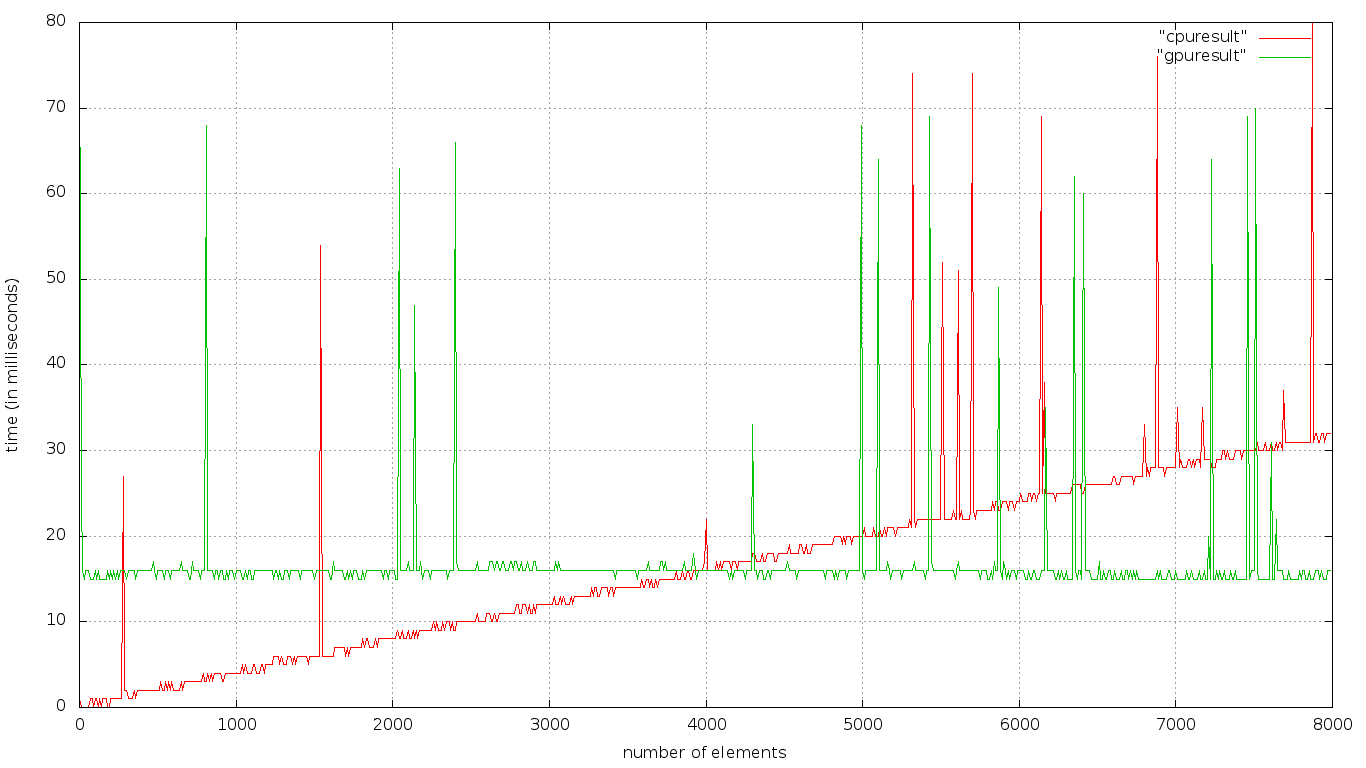
\includegraphics [width=1.2\textwidth]{plot1.png}

\section{Inferences}
\begin{enumerate}
\item When this code is run, you will find that the CPU is faster than the GPU for an array of 3,900 elements. If you increase the size to 3,900 to about 4,000 elements in the array, the two will essentially tie. Above 4,000 elements in the array, and the GPU will win. 
\item The threads should be running in groups of at least 32 (since the kernel issues commands equal to the warp size [32 in our case]) for best performance, with total number of threads numbering in the thousands. Branches in the program code do not impact performance significantly, provided that each of 32 threads takes the same execution path; the SIMD execution model becomes a significant limitation for any inherently divergent task.
\item The overhead in creating threads on GPU kernel remains same, it does not depends on the number of elements. 
\end{enumerate}


\chapter{Benchmark-III}

\section{The Task}
The objective of the program is simple. It’s the brute force euclidian distance transform. Basically, in a binary image, for each pixel in the foreground we verify what is the 2D euclidian distance to the nearest pixel in the background.

\section{Code Walkthrough}
Code Walkthrough mentioned in file codewalkthrough.
\section{Result}
\subsection{Output}
It took about 35.8 seconds for a 1 megapixel image in a Tesla C2050 GPU and about 1 hour on normal CPU.\\\\
\newpage
\subsection{Images}
\vspace{1cm}
\textbf{Input Image}\\\\
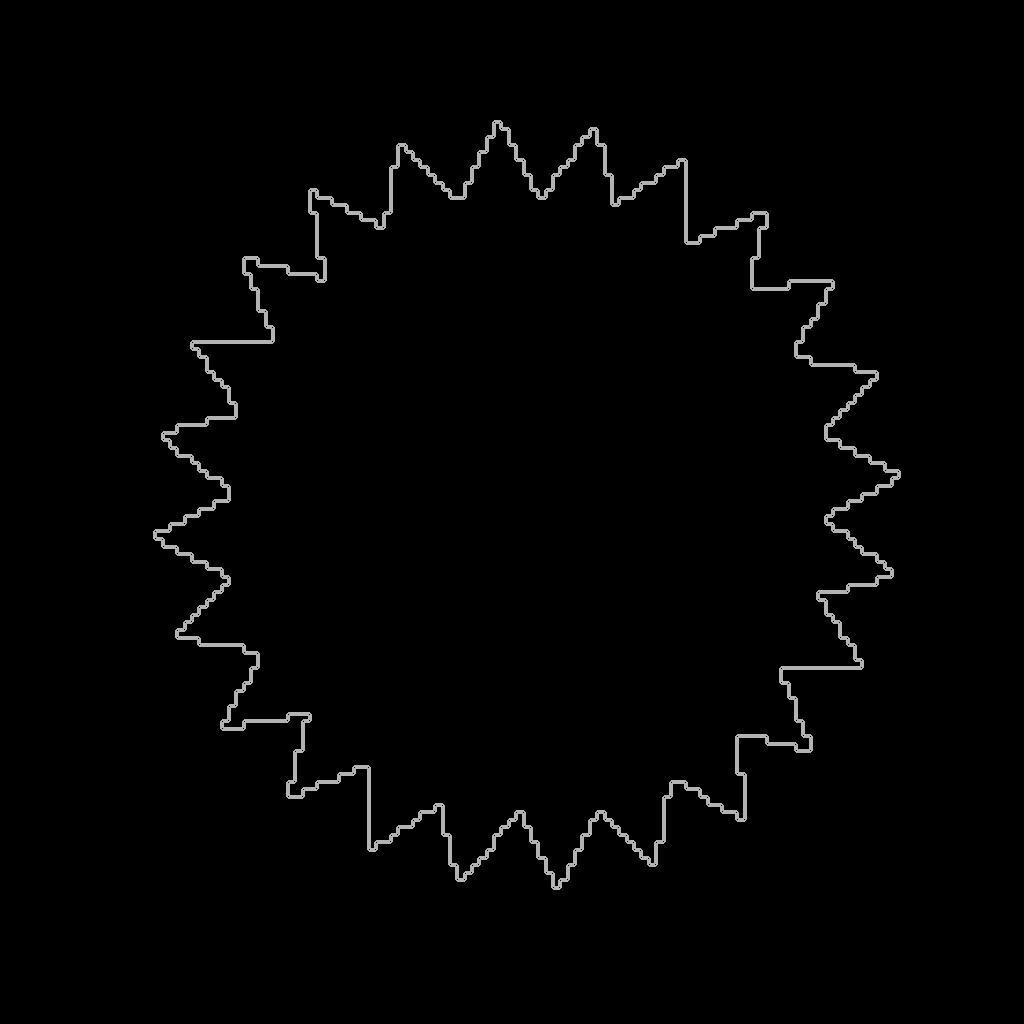
\includegraphics [width=1.2\textwidth]{input.png}
\newpage
\textbf{Output Image}\\\\

\includegraphics [width=1.2\textwidth]{output.png}

\section{Inferences}
\begin{itemize}
\item From this it could be inferred that brute force ran fast on GPU rather than CPU. 
\end{itemize}

\newpage
\chapter{Benchmark-IV}

\section{The Task}
\textbf{What is Video Rendering}\\\\
Rendering is the computer's way of taking effects, such as color correction or transitions, and adding them to the actual video in order to make the video playback smooth. Without the rendering process, the video playback would be choppy because the computer would have to compute the video and the effects separately.\\\\
\textbf{Benchmarking GPU Acceleration in Vegas Pro 12}\\\\
Vegas Pro™ 12 leverages the processing capabilities of modern GPUs (Graphic Processing Units) using the industry-standard OpenCL™ framework. Rather than being tied to a single manufacturer or technology, this hardware-agnostic approach enables Vegas Pro 12 users to enjoy remarkable performance improvements across a broad range of popularly-priced, widely available GPU devices. By utilizing the amazing parallel computing resources of the GPU for video processing, the main CPU is freed up for other tasks, such as video decoding and user interface display.\\
Vegas Pro 12 accelerates both video playback and rendering, providing improved performance results from start to finish. Significant portions of the application were entirely reworked, resulting in an enhanced and more creative editing experience. Over 45 effects, transitions, generators and compositors are GPU-accelerated in Vegas Pro 12, as well as a substantial amount of built-in video processing such as crossfades, fades, alpha compositing, framerate resampling, interlace processing, pan/crop, track motion, opacity, fade-to-color, and multicamera display.\\
\section{Results}
\textbf{Video Details:}\\
	Video Resolution: 1920 x 1080\\
	fps: 29\\
	filetype: NTSC-mp4\\
	Playback Time: 6:47 min\\\\
\textbf{Intel Xeon with Nvidia Tesla C2050}\\
	Rendering Time: 5:40 min\\
	Output format: Mainconcept Internet HD 1080p (mp4)\\
	CPU Usage : 70-75\%\\
	GPU Usage : 60-70\%\\\\
\textbf{Intel Xeon without Nvidia Tesla C2050}\\
	Rendering Time: 19:34 min\\
	Output format: Mainconcept Internet HD 1080p (mp4)\\
	CPU Usage : 90-95\%\\
	GPU Usage : None\\\\
\textbf{Intel i5-2450M with Nvidia Geforce GT 525m}\\ 
	Rendering Time: 16:18 min\\
	Output format: Mainconcept Internet HD 1080p (mp4)\\
	CPU Usage : 70-75\%\\
	GPU Usage : 60-70\%\\\\
\textbf{Intel i7-3610QM with Nvidia Geforce GT 630m}\\ 
	Rendering Time:  9:01 min\\
	Output format: Mainconcept Internet HD 1080p (mp4)\\
	CPU Usage : 25-35\%\\
	GPU Usage : 85-90\%\\\\\\

\newpage
\section{Output}
\textbf{Intel Xeon with Nvidia Tesla C2050}\\\\
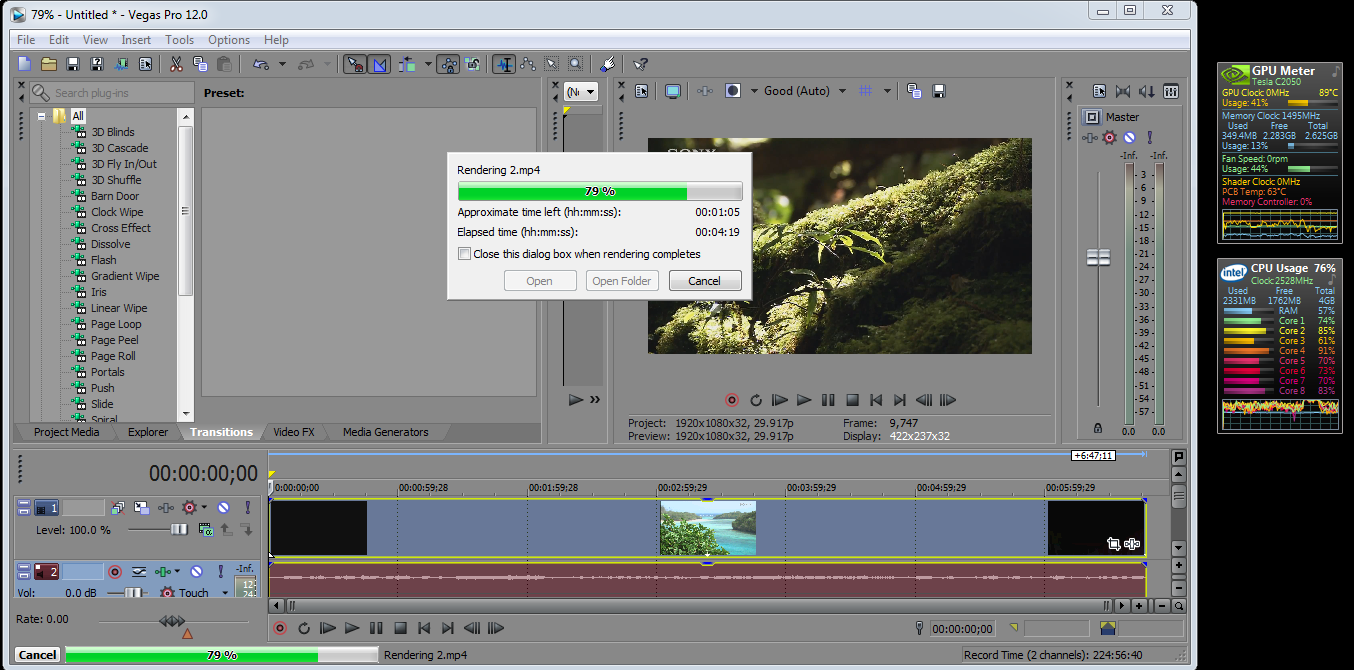
\includegraphics [width=1.2\textwidth]{sony1.png}
\newpage
\textbf{Intel i5-2450M with Nvidia Geforce GT 525m}\\\\
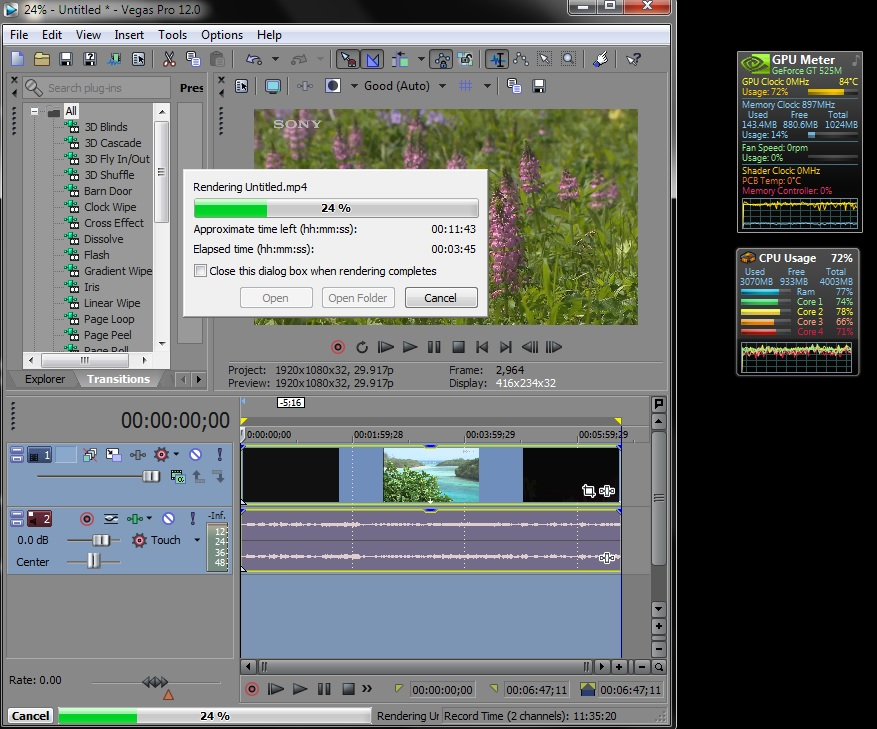
\includegraphics [width=1.2\textwidth]{525m.jpg}\\
\newpage
\textbf{Intel i7-3610QM with Nvidia Geforce GT 630m}\\\\
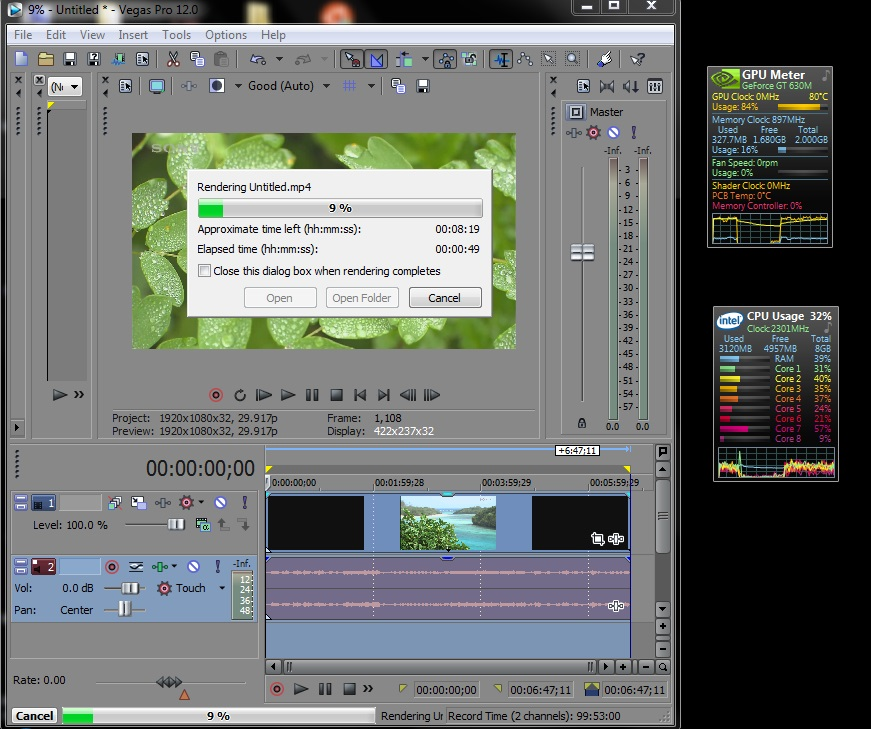
\includegraphics [width=1.2\textwidth]{630m.jpg}


\chapter{Bottlenecks}
\begin{enumerate}
\item Copying between host and device memory may incur a performance hit due to system bus bandwidth and latency (this can be partly alleviated with asynchronous memory transfers, handled by the GPU's DMA engine)
\item Threads should be running in groups of at least 32 for best performance, with total number of threads numbering in the thousands. Branches in the program code do not impact performance significantly, provided that each of 32 threads takes the same execution path; the SIMD execution model becomes a significant limitation for any inherently divergent task 
\item Consider we have an application in which we need to create an array that has 20,000 integers. So the amount of memory we will need to fit 20,000 integers = 20,000 * 4B = 80KB. But the maximum amount of shared memory per multiprocessor is 48 KB.
\item For a large number of threads, we can't assign more than 1024 threads per block.
\item Local memory being limited to 512 KB could hurt the performance in two ways-
\begin{enumerate}
\item Increased pressure on the memory bus
\item Increased instruction count
\end{enumerate}
\end{enumerate}

\chapter{Conclusion}

\section{Project Status}
\begin{itemize}
\item The project is not complete in its entireity as a lot more modules can be implemented. We tried to implement the Brute Force technique but due to time boundation we were not able to implement it.
\item Some of the benchmarking tools could not be implemented due to insufficient resources.
\end{itemize}

\section{Future Intentions with the project}
\begin{itemize}
\item It has been quite a learning process and the project made can surely undergo a lot of modifications to become a well equipped parallelizer.
\item We would continue this to make sure that Brute Force (MD5 Hashing) is implemented and a bit of more study of how can this be improved would be done.
\end{itemize}

%-----------------------------------------------------------
%\begin{thebibliography}{9999}

\bibitem[AC]{AC}A~Cottrell, \textsl{Word Processors: Stupid and
Inefficient},
\\ \mbox{}\hfill\texttt{www.ecn.wfu.edu/\~{}cottrell/wp.html}

\bibitem[BR]{BR}Visit \texttt{www.dur.ac.uk/library/using/guides/}
and click on \Quote{Writing your bibliography and citing references}.

\bibitem[ESL]{ESL}L~Truss, \textsl{Eats, Shoots and Leaves}, Profile
  Books 2003\\ \mbox{}\hfill(ISBN~\texttt{1-86197-612-7}).

\bibitem[GRM]{GRM}M~Goossens, S~Rahtz and F~Mittelbach,\\
  \mbox{}\hfill \textsl{The \LaTeX\ Graphics Companion},
  Addison-Wesley, 1997\\  \mbox{}\hfill(ISBN~\texttt{0-201-85469-4}).

\bibitem[IM]{IM} \textsl{ImageMagick}, {\tt%
www.dur.ac.uk/its/software/application/\dots
\\ \mbox{}\hfill\dots?application=ImageMagick}

\bibitem[LAT]{LAT} \textsl{\LaTeX\ stuff},
	\texttt{maths.dur.ac.uk/Ug/projects/resources/latex/}

\bibitem[MEM]{MEM} \textsl{Memoir document class},\\ \mbox{}\hfill
   \texttt{www.ctan.org/tex-archive/macros/latex/contrib/memoir/}

\bibitem[MG]{MG}F~Mittelbach and M~Goossens \etal, \textsl{The
\LaTeX\ Companion},\\  \mbox{}\hfill Addison-Wesley, 2nd ed. 2004
(ISBN~\texttt{0-201-36229-6}).

\bibitem[MKT]{MKT} \textsl{MikTex Project Page}, \texttt{www.miktex.org}

\bibitem[NSS]{NSS}T~Oetiker, H~Partl, I~Hyna and E~Schlegl,\\
\mbox{}\hfill
\textsl{The Not So Short Introduction to \LaTeXe},\\ \mbox{}\hfill{\tt
www.ctan.org/tex-archive/info/short}

\bibitem[PS]{PS} \textsl{Photoshop}, {\tt%
www.dur.ac.uk/its/software/application/\dots
\\ \mbox{}\hfill\dots?application=Adobe+Photoshop}

\bibitem[TXC]{TXC} \textsl{TeXnicCenter}, \texttt{www.toolscenter.org}

\bibitem[WDT]{WDT} \textsl{WinEdt}, \texttt{www.winedt.com}

\bibitem[WL]{WL} \textsl{Wikibook on \LaTeX}, \texttt{%
	en.wikibooks.org/wiki/Latex}
\bibitem[WO]{WO} \textsl{Controlling widows and orphans}, 
\\ \mbox{}\hfill\texttt{www.tex.ac.uk/cgi-bin/texfaq2html?label=widows}
\bibitem[WSH]{WSH} \textsl{WinShell}, \texttt{www.winshell.de}
\end{thebibliography}
\vfill
\begin{flushright}\small Prepared in \LaTeXe\ by RCJ\end{flushright}

%-----------------------------------------------------------
\end{document}
